\begin{frame}
\frametitle{}
\hspace*{-1.2cm}
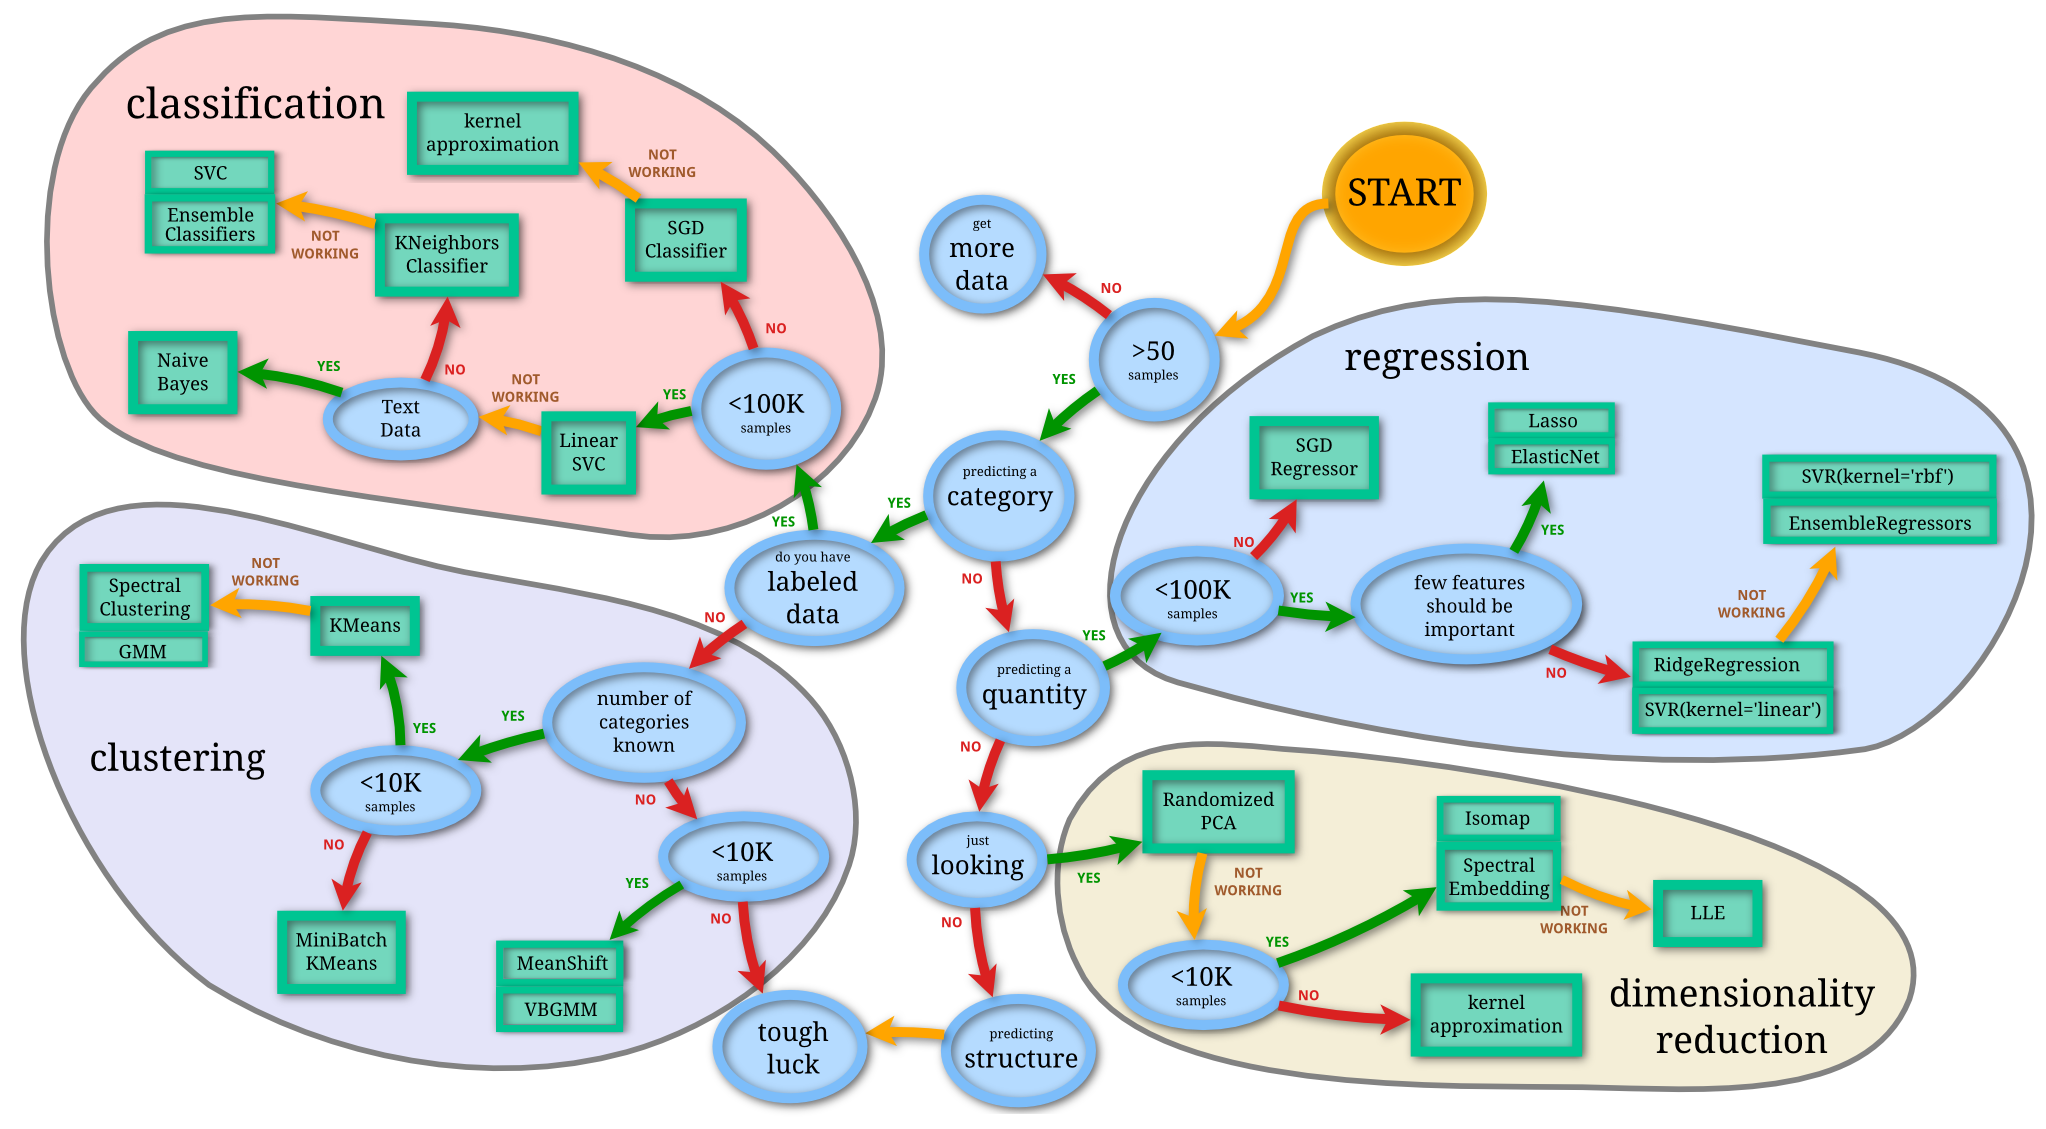
\includegraphics[width=1.2\textwidth]{sklearn_material/overview.png}
% Note: need some adaptation. Should not be sklearn specific
% useful to clarify the different branches of ML
% 
\end{frame}


\begin{frame}
\frametitle{Some key concepts}



\textbf{supervised learning}: the data comes with additional
attributes that we want to predict $\Longrightarrow$
classification and regression.\\
\vspace{1cm}

\textbf{unsupervised learning}: no target values. 
\begin{itemize}
\item
discover groups of similar examples within the data (clustering)
\item
determine the distribution of data within the input space (density estimation)
\item
project the data down to two or three dimensions for visualization
\end{itemize}

\end{frame}



